\section{Opis implementacji algorytmu \texttt{RRT} \label{sec:rrt_impl}}
W trakcie testów wersji podstawowej algorytmu \textit{RRT} opisanej w \ref{sec:RRT:basic} zdecydowano się na dodatkowe modyfikacje algorytmu, część zaczerpnięto z 
\ref{sec:RRT:extend} dodano też własne modyfikacje, które miały na celu poprawienie wydajności algorytmu i skrócenie czasu obliczeń.
Zdecydowano się na implementację algorytmu w wersji z zapamiętywaniem części węzłów ze ścieżki wyznaczonej w poprzednim uruchomieniu algorytmu (pod warunkiem, że punkt docelowy nie
uległ zmianie) i traktowanie ich jako tak zwanych \texttt{way points}. Jednak z uwagi na specyfikę eksplorowanego środowiska (brak wąskich korytarzy, przeszkody są wypukłe)
zdecydowano się na eliminowanie z zapamiętanej ścieżki węzłów których odległość między sąsiadami jest mniejsza niż $5cm$. Zrezygnowano z przechowywania węzłów w postaci \texttt{KD-drzewa}.

Dodatkowo wprowadzono ograniczenie na maksymalną liczbę węzłów algorytmu. Sytuacja na planszy podczas rozgrywki szybko ulega zmianie, stąd wyznaczanie kompletnej 
ścieżki do celu pozbawione jest sensu, jeśli ma to być czasochłonne. Przy ponownym uruchomieniu algorytmu sytuacja może wyglądać inaczej i algorytm szybciej wyznaczy ścieżkę.
Jeśli uruchomienie algorytmu nie zakończyło się wyznaczeniem kompletnej ścieżki do celu jako punkt docelowy dla robota wybierany jest węzeł znajdujący się najbliżej celu.

Zauważono także, że przy małym prawdopodobieństwie budowy ścieżki do celu, drzewo może ulegać nadmiernemu rozbudowaniu przy samym korzeniu. Ma to miejsce w sytuacji, gdy
tymczasowe punkty losowane są z otoczenia korzenia, kolejne wylosowane węzły mogą powodować poszerzenie gałęzi, a tak rozbudowane gałęzie mogą znajdować się w podobnej 
odległości od celu. W efekcie algorytm przez dłuższy czas może próbować wyznaczać kilka ścieżek prowadzących do celu, co nie jest pożądane. Sytuację taką dla dwóch gałęzi przedstawiono na rysunku \ref{fig:many_root_child}.
\begin{figure}[h]
\centering
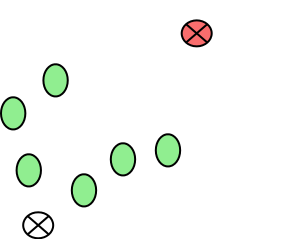
\includegraphics[scale=0.5]{./imp_rrt/many_root_child.png}
\caption{ Drzewo wyznaczające ścieżkę do celu.} \label{fig:many_root_child}
\end{figure} 
W zaimplementowanej wersji ograniczono liczbę wezłów potomnych korzenia do $4$.

Podobnie jak w pracy inżynierskiej \cite{inzynierka} zdecydowano się na naiwną predykcję położenia dynamicznych przeszkód. Ponieważ baza jezdna robota zbliżona jest do okręgu
w algorytmie jest ona analizowana jako okrąg o środku znajdującym się w danym położeniu robota (przeszkody) i promieniu $r=2*(r_{base} + l_{dribbler})$, gdzie $r_{base}$ jest
promieniem bazy jezdnej robota, a $l_{dribbler}$ długością dribblera.
Do zbioru rzeczywistych przeszkód dodawne są przeszkody, których  środek przesunięty jest o drogę jaką może pokonać dana przeszkoda w czasie trwania jednego uruchomienia algorytmu.
Podczas planowania ścieżki promienie przeszkód powiększane są dodatkowo o margines bezpieczeństwa, ma on za zadanie wyeliminowanie ewentualnych kolizji wynikających z poślizgu robota
podczas hamowania, czy opóźnienia przy zmianie kierunku jazdy. Główną zaletą \texttt{RRT} jest jego szybkość, stąd przewidywanie położenia przeszkody na $1$ krok w przód okazało
się wystarczające. W przypadku \texttt{CVM} konieczne było dodawanie ``wirtualnych'' przeszkód symulujących położenie robotów za $15$, $30$ oraz $45$ kroków symulatora. 

W zaimplementowanej formie algorytm ma następujący przebieg:
  \begin{algorithm}[H]
	\caption{ Wersja \texttt{RRT} z wprowadzonymi modyfikacjami }
	\label{alg:myRRT}
	\begin{algorithmic}
	\STATE ogranicz maksymalną przestrzeń do rozmiarów boiska
	\IF{punkt docelowy jest poza dopuszczalnymi współrzędnymi} \STATE zwróć błąd \textit{waypoints} \ENDIF
	\IF{w poprzednim uruchomieniu znaleziono ścieżkę do celu} \STATE zainicjuj listę \textit{waypoints} \ENDIF
	\STATE dodaj statyczne oraz dynamiczne przeszkody;
	\IF{robot uległ kolizji (nie są brane pod uwagę przewidywane położenia przeszkód)} \STATE tak zwróć błąd;\ENDIF
	\IF{robot dojechał do celu} \STATE tak zwróć sukces;\ENDIF
	\IF{punkt docelowy jest w obrębie przeszkody} \STATE zwróć błąd;\ENDIF
	\IF{punkt docelowy jest bezpośrednio osiągalny} \STATE zwróć go jako wynik działania algorytmu;\ENDIF
	\WHILE { \texttt{goalState.distance(nextState)} $>$ \texttt{minimalDistance}
	  \&\& \texttt{treeSize}< \texttt{maxNodeNumber} }
	  \STATE wybierz tymczasowy cel: \texttt{tmp\_target} =  \texttt{chooseTarget(goalState)}
	  \STATE nearestState $=$ \texttt{ nearest(tree, target) }
	  \STATE \texttt{extendedState} $=$ \texttt{extend(env, nearest, target)}
	  \IF { \texttt{extendedState} $!=$ \texttt{NULL} }
	    \STATE odblokuj ustawianie \texttt{tmp\_target} jako texttt{goalState}
	    \STATE \texttt{addNode(tree, extended)}
	  \ELSIF{ \texttt{tmp\_target} należy do zbioru \textit{waypoints}}
	    \STATE usuń punkt ze zbioru \textit{waypoints}
	  \ELSIF{ \texttt{tmp\_target} jest właściwym punktem docelowym}
	    \STATE zablokuj ustawianie \texttt{tmp\_target} jako texttt{goalState}
	  \ENDIF
	\ENDWHILE
	\IF { \texttt{nearestState.distance(goalState)} $>$ \texttt{minimalDistance} }
	\RETURN węzeł znajdujący się najbliżej celu
	\ELSE
	  \STATE zapamiętaj ścieżkę do celu
	  \RETURN  węzeł bezpośrednio osiągalny znajdujący się najbliżej celu;
	\ENDIF 
	\end{algorithmic}
  \end{algorithm}

W opisie algorytmu zastosowano fukcje \texttt{chooseTarget} oraz \texttt{extend}, których działanie również zostało lekko zmodyfikowane w stosunku do oryginalnej
wersji algorytmu. Ich działanie zostało przedstawione poniżej: 
 \begin{algorithm}[H]
	\caption{ funckcja \texttt{chooseTarget} wyznaczająca tymczasowy punkt docelowy }
	\label{alg:mychooseTarget}
	\begin{algorithmic}
	\STATE \texttt{function} \textit{chooseTarget}(\textit{goal:state}) \textit{state};
	\STATE p = \texttt{uniformRandom in}$[0.0 ...1.0]$
	\IF{wyznaczono ścieżkę w poprzednim uruchomieniu algorytmu}
	  \IF{$0.0<p<goalProb$}
	    \IF{wybór właściwego punktu docelowego jest zablokowany}
	      \RETURN  \texttt{randomPoint};
	    \ENDIF 
	    \RETURN  właściwy punkt docelowy
	  \ELSIF{ $p<goalProb+wayPointProb$}
	    \STATE i = \texttt{uniformRandom in}$[0 ...number\_of\_waypoints -1]$
	    \RETURN \textit{WayPoints[i]}
	  \ELSE
	    \RETURN \textit{RandomState()}
	  \ENDIF
	\ELSE
	  \IF{$0.0<p<goalProb$ \&\& wybór właściwego punktu docelowego nie jest zablokowany } 
	    \RETURN  \texttt{goal};
	  \ELSE
	    \RETURN \textit{RandomState()}
	  \ENDIF
	\ENDIF
	\end{algorithmic}
  \end{algorithm}

 \begin{algorithm}[H]
	\caption{ funckcja \texttt{extend(nearest,tmp\_target)} rozszerzejąca drzewo w kierunku zadanego punktu }
	\label{alg:myextend}
	\begin{algorithmic}
	\STATE podczas detekcji kolizji przeszkody powiekszane są o margines bezpieczeństwa
	oraz uwzględniane są dodatkowe przeszkody wynikające z ruchu robotów
	\IF{punkt docelowy leży w obrębie przeszkody}
	  \RETURN \texttt{NULL}
	\ENDIF
	\STATE wyznacz nowy węzeł (\texttt{newNode}) odległy od \texttt{nearest} w kierunku \texttt{tmp\_target}
	\IF{ wyznaczony punkt leży w obrębie przeszkody}
	  \RETURN \texttt{NULL}
	\ENDIF
	\RETURN \texttt{newNode}
	\end{algorithmic}
  \end{algorithm}

\subsection{Parametry zastosowanego algorytmu}
Zaimplementowowaną wersję algorytmu \texttt{RRT} można w łatwy sposób konfigurować poprzez zmiane kluczowych parametrów takich jak: 
\begin{enumerate}
 \item włączanie/wyłączanie predykcji ruchu przeszkod,
 %\item rodzaj metody do predykcji ruchu przesuniete okręgi/ilosc okregow /elipsa 
 \item prawdopodobieństwo losowania tymczasowego punktu docelowego należącego do \texttt{wayPoints} (\textit{goalProb}) lub jak punkt docelowy \textit{wayPointProb},
 \item rozmiary dopuszczalnej przestrzeni z jakiej losowany jest tymczasowy cel, wynikajace z rozmiaru swiata,
 \item ograniczenia na przestrzen przeszukiwan wynikajace z zaistnialej sytuacji na planszy, bądź z rodzaju zadania,
 \item odległości po przekroczeniu której uznajemy, że robot dojechał do celu,
 \item ścieżka z poprzedniego wywołania algorytmu, przekazywana tylko wtedy gdy punkt docelowy nie zmienił się,
 \item maksymalna liczba węzłów drzewa \texttt{RRT},
 \item maksymalna liczba węzłów doczepionych do korzenia,
 \item odległość między \texttt{wayPoints}; z przekazanej ścieżki scalane są te między którymi odległość jest mniejsza niż wartość parametru,
 \item \textit{rrtStep} odległość o jaką rozszerzany jest węzeł leżący najbliżej tymczasowego celu w jego kierunku,
 \item odleglość punktu startowego od najbliższej przeszkody, brane są pod uwagę jedynie bieżące położenia robotów. 
\end{enumerate}